% =============================================================================
% midcenturymodern_demo.tex
% Demo file for the Mid-Century Modern Beamer template.
% Compile with: lualatex midcenturymodern_demo.tex
% =============================================================================
\documentclass[aspectratio=169]{beamer}
\usepackage{beamerthememidcenturymodern}
\usepackage[backend=biber, style=authoryear, sorting=nyt]{biblatex}
\addbibresource{demo.bib}

% --- Theme selection (comment/uncomment to switch) ---
\mcmTheme{Kraft}
% \mcmTheme{DeepBlue}
 % 
% --- Metadata ---

\institute{Singapore Nuclear Research and Safety Institute}


\titlegraphic{
  \begin{minipage}{0.21\linewidth}
    \begin{center}

    \end{center}
  \end{minipage}
}

% --- Automatic section/subsection pages ---
\AtBeginSection[]{%
  \begin{frame}[plain]
    \sectionpage
  \end{frame}
}
\AtBeginSubsection[]{%
  \begin{frame}[plain]
    \subsectionpage
  \end{frame}
}

\AtEveryCite{\color{mcmPrimary}}

% Use a clean, modern theme. You can swap this with your preferred template later.

\usepackage{graphicx}
\usepackage{amsmath}
\usepackage{booktabs}

% Title Information
\title[Point Reactor Kinetics Equations]{FHR Operations Challenge}
\subtitle{An Introduction to Reactor Dynamics}
\author{Dr Theodore Ong, SNRSI, NUS}
\date{\today}

\begin{document}

% --- Slide 1: Title Slide ---
\begin{frame}
    \titlepage
\end{frame}

% --- Slide 2: The Mission Briefing ---
\begin{frame}{Mission Briefing: Grid Demand Increase}
    \begin{columns}
        \begin{column}{0.6\textwidth}
            Currently, our Fluoride-salt-cooled High-temperature Reactor (FHR) is operating stably, supplying baseload power to the grid.

            \vspace{1em}

            \textbf{The Situation:}
            Grid demand has just spiked. The grid operator requests an immediate increase in power output.

            \vspace{1em}

            \begin{alertblock}{Your Objective}
                Increase reactor thermal power from \textbf{30 MWth} to \textbf{60 MWth} and stabilize it there.
            \end{alertblock}
        \end{column}
        \begin{column}{0.4\textwidth}
            \centering
            % Replace with a generic reactor icon or relevant image if desired
			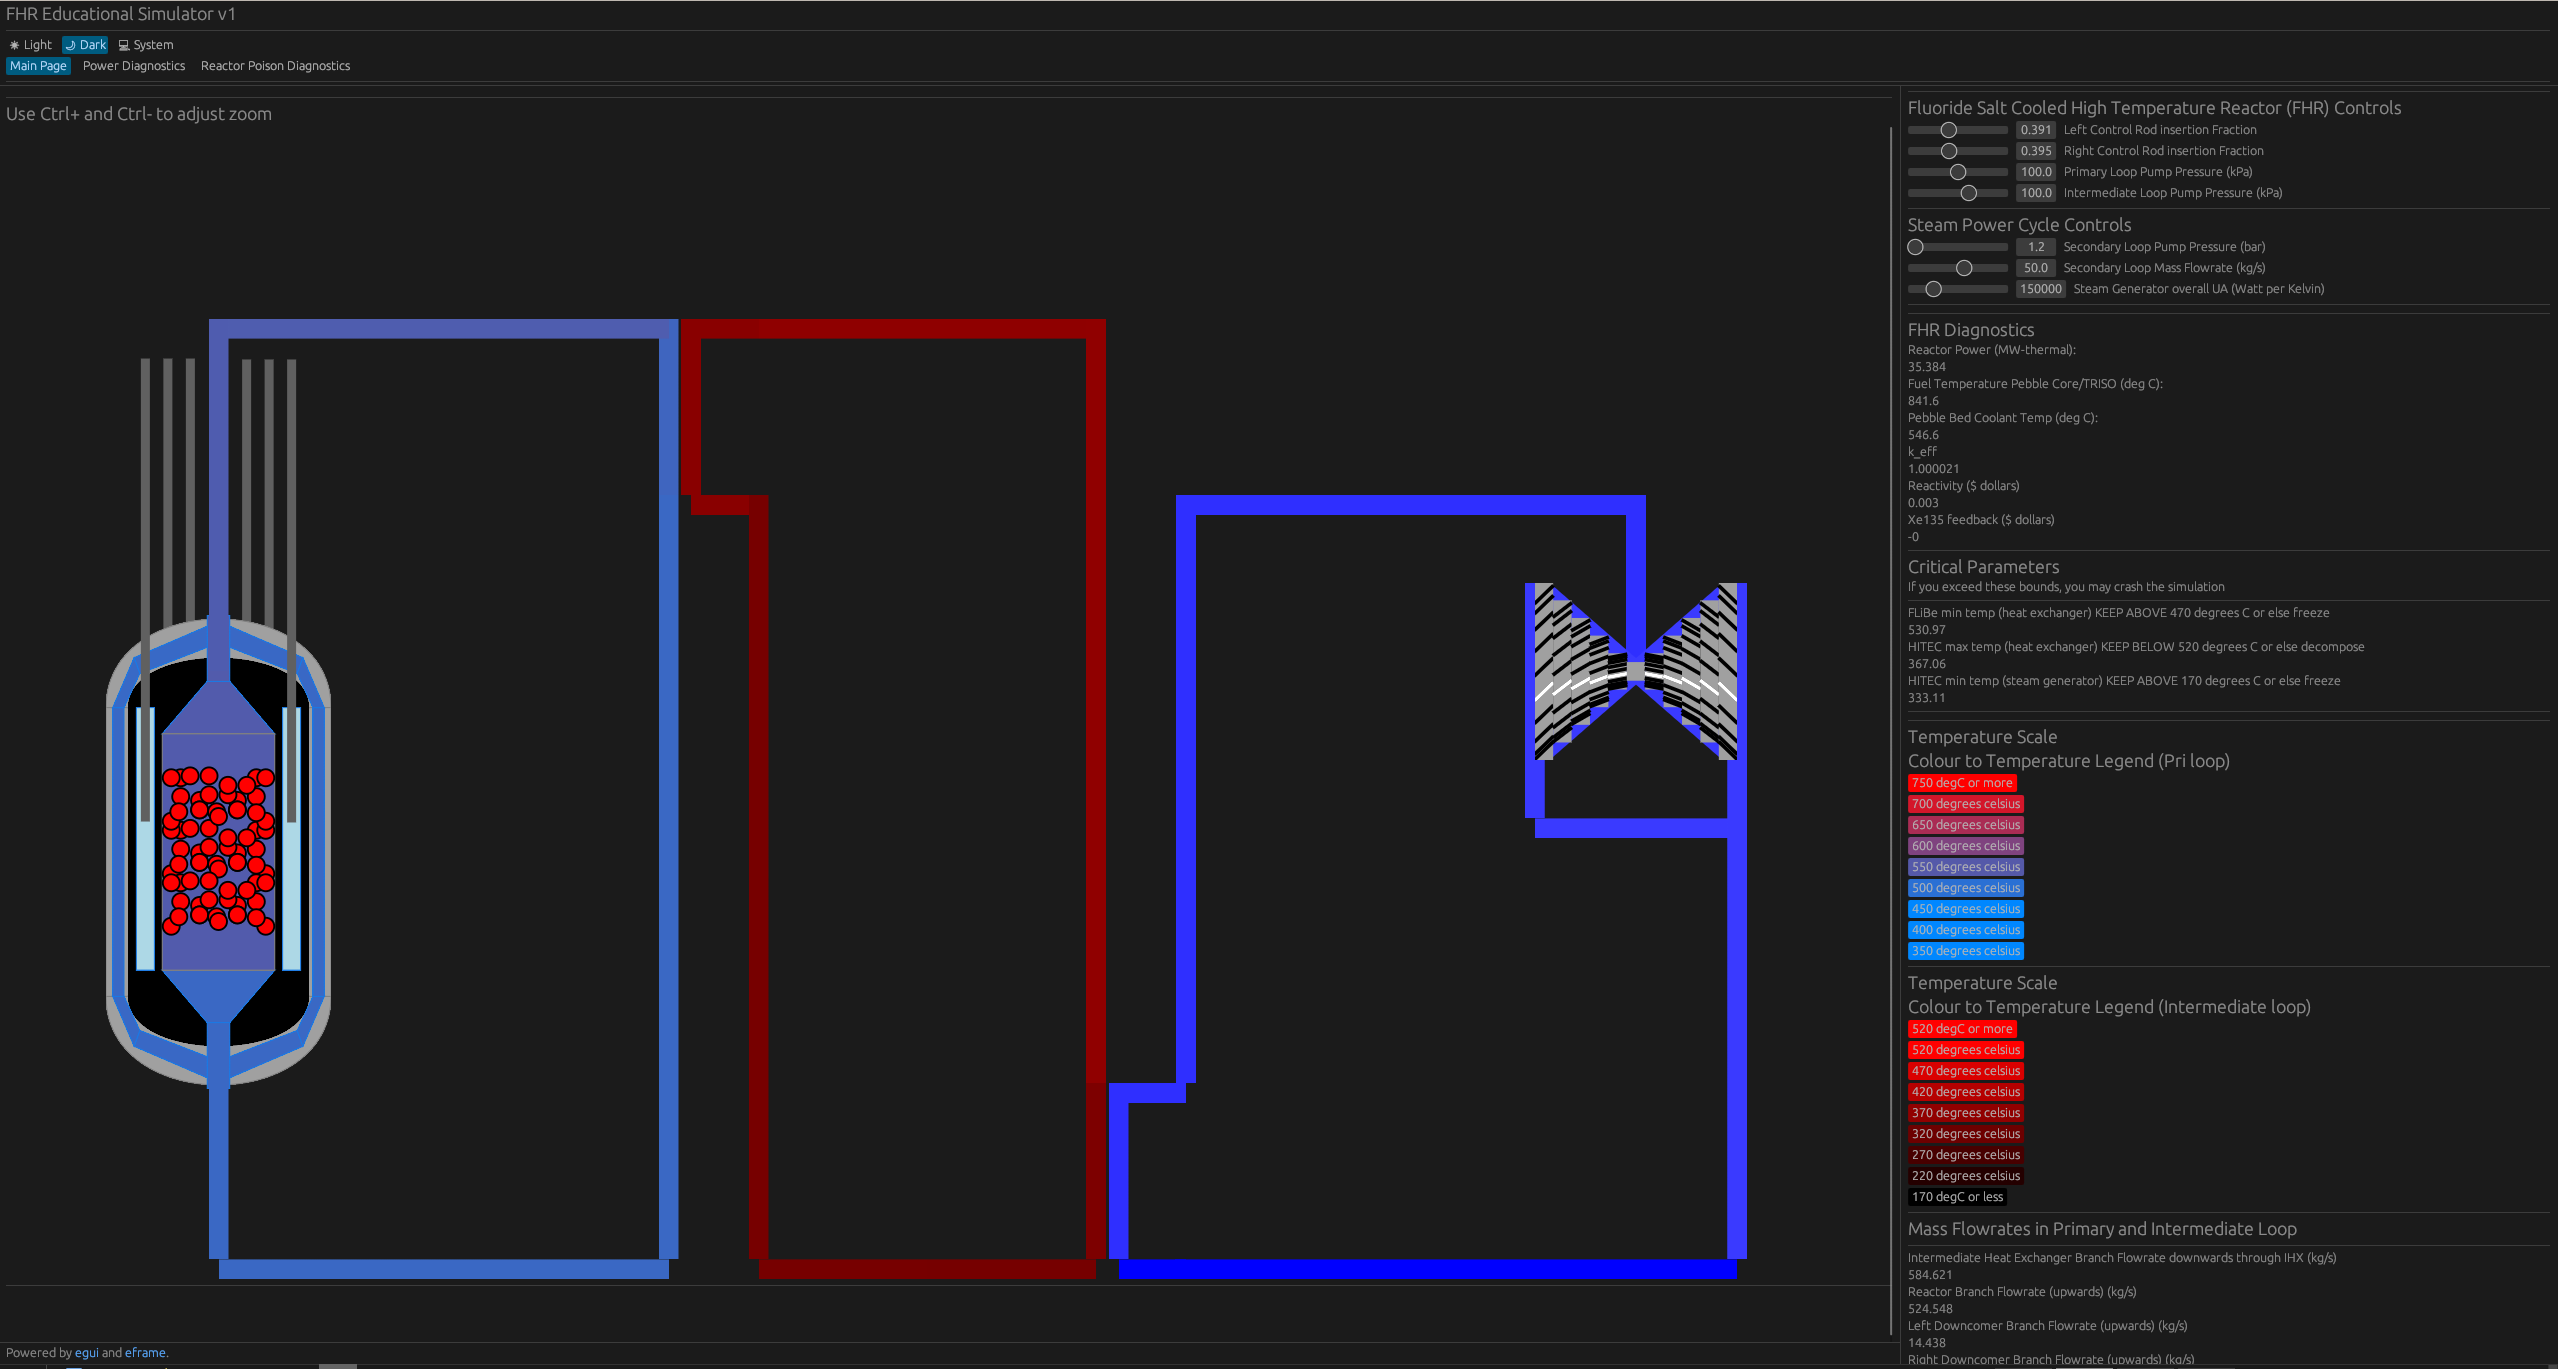
\includegraphics[width=0.8\textwidth]{./fhr_sim_full.png} 
        \end{column}
    \end{columns}
\end{frame}

% --- Slide 3: Operational Constraints ---
\begin{frame}{Operational Constraints \& Safety Limits}
    Nuclear reactors are powerful systems that require precise control. We cannot just "floor the accelerator."

    \vspace{1em}

    \textbf{The Rules of Engagement:}
    \begin{itemize}
        \item You have full control over the reactor's control rods (reactivity).
        \item You must aim for exactly \textbf{60 MWth}.
    \end{itemize}

    \vspace{2em}

    \begin{block}{SAFETY LIMIT (FAILURE CONDITION)}
        If reactor power exceeds \textbf{1000 MWth} at any point during the maneuver, you have violated the reactor's safety limits and failed the mission.
    \end{block}
\end{frame}

% --- Slide 4: Simulator Interface Overview (Placeholder) ---
% INSTRUCTION: Replace 'example-image' with a screenshot of your FHR simulator
% showing the power gauge, reactivity controls, and main readout at 30 MWth.
\begin{frame}{Your Interface: The FHR Control Panel}
    \centering
	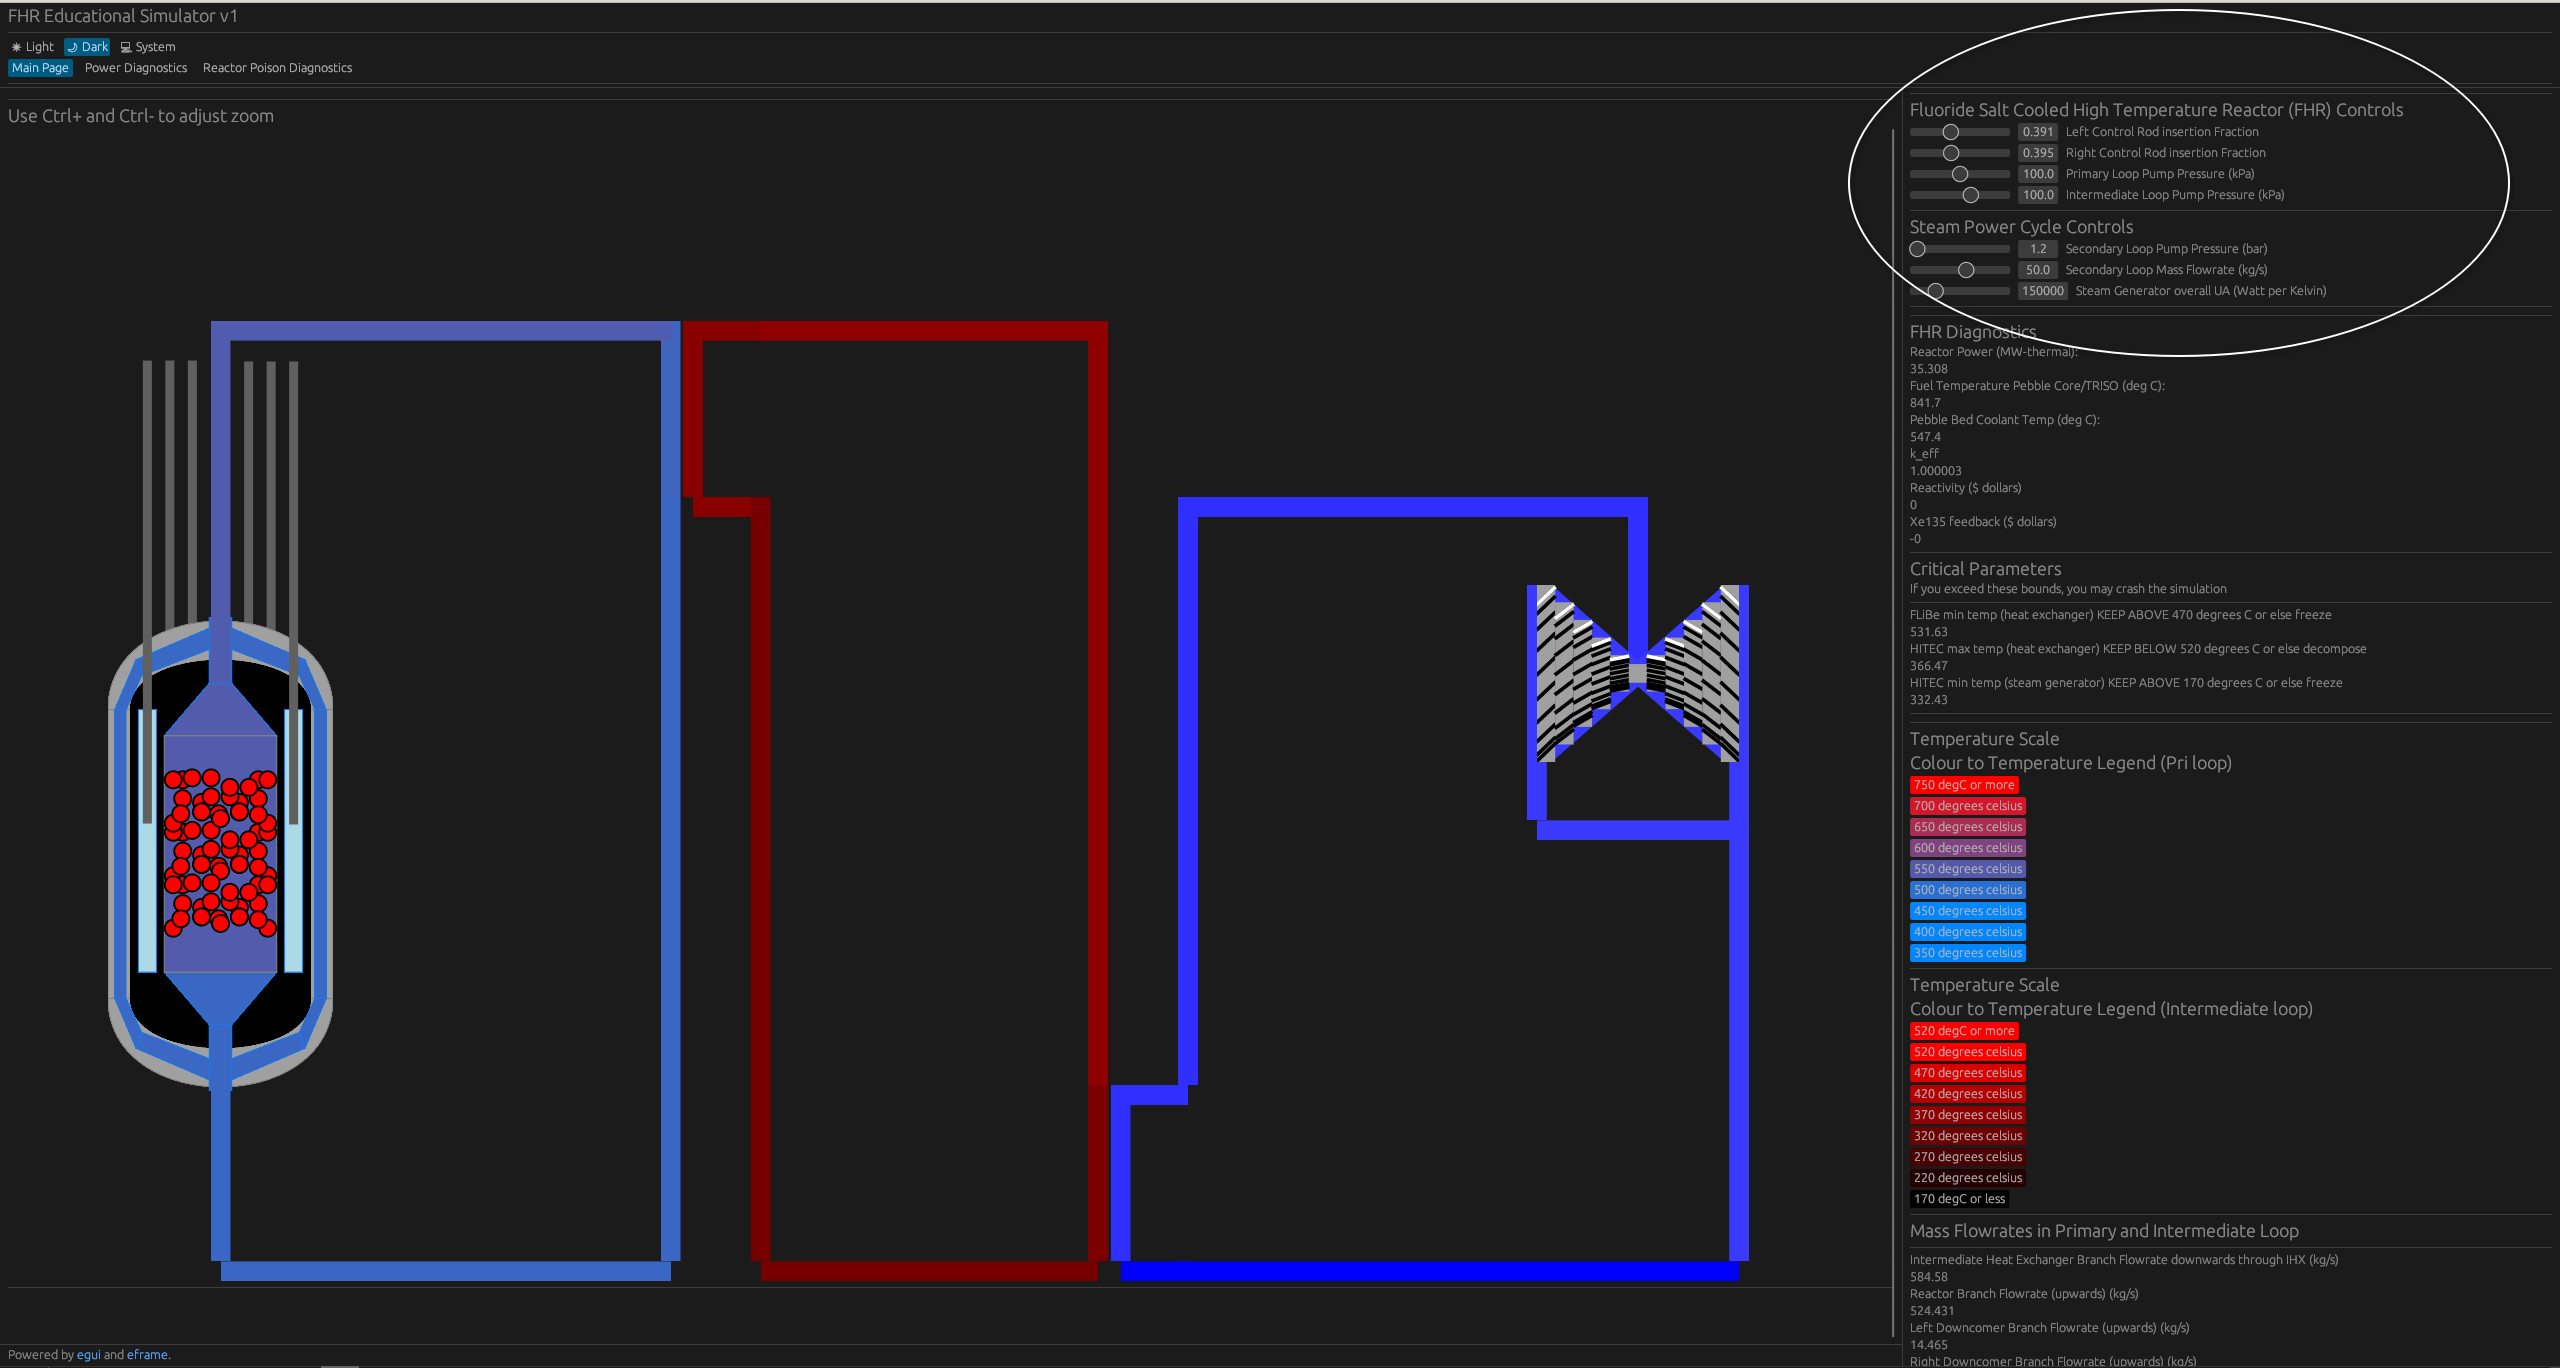
\includegraphics[width=0.85\textwidth, keepaspectratio]{./fhr_sim_controls.png}
    \vspace{0.5em}
    \footnotesize{\textit{Current State: Stable at 30 MWth}}
\end{frame}

% --- Slide 5: The Challenge Begins (While students attempt) ---
\begin{frame}{The Challenge Begins}
    \centering
    \Huge \textbf{Volunteers Needed!}

    \vspace{2em}
    \normalsize
    Who thinks they have the steady hand to bring us to 60 MWth without exceeding 1000 MWth?

    \vspace{2em}
    \hrule
    \vspace{1em}

    \textbf{For the rest of the class (Observers):}
    Watch closely. Don't just look at the power level.
    \begin{itemize}
        \item How does the reactor respond immediately after they move the controls?
        \item What happens to the power when they \textit{stop} moving the controls?
        \item Does the reactor feel "heavy" (slow to move) or "twitchy" (fast to move)?
    \end{itemize}
\end{frame}

% --- Slide 6: Debrief (After 2-3 attempts) ---
\begin{frame}{Debrief: Intuition vs. Reality}
    We just saw a few attempts. It wasn't as easy as turning up a volume knob on a radio.

    \vspace{1em}

    \textbf{Discussion Questions:}
    \begin{enumerate}
        \item Did anyone overshoot the 60 MWth target? Why did that happen?
        \item Did you notice the power continuing to change even after you put the controls back to neutral?
        \item If you added too much reactivity, did it feel like the reactor was "running away" from you?
    \end{enumerate}

    \vspace{1em}
    \begin{center}
        \textbf{Why does the reactor have "momentum"? Why doesn't it stop instantly?}
        
        \textit{To answer this, we need to look at the physics of neutron populations.}
    \end{center}
\end{frame}

% --- Slide 7: Transition to Theory ---
\begin{frame}{The Hidden Mechanism}
    You experienced the reactor's behavior:
    \begin{itemize}
        \item It doesn't respond instantly to control rod changes.
        \item It has "momentum" – power keeps changing after you stop acting.
        \item If you add too much reactivity quickly, it feels uncontrollable.
    \end{itemize}

    \vspace{2em}
    \centering
    \textbf{To understand why, we need to look at the life cycle of neutrons.}
    
    We use the \textbf{Point Reactor Kinetics Equations (PRKE)} to model this.
\end{frame}

% --- Slide 8: The Foundation - Neutron Balance ---
\begin{frame}{Step 1: The Neutron Balance}
    At its simplest, reactor power changes based on the population of neutrons ($n$) \cite{bell1970nuclear}.

    $$ \text{Rate of Change} = \text{Production} - \text{Loss} $$
    $$ \frac{dn}{dt} = \text{Production} - \text{Loss} $$

    \vspace{1em}
    The production and loss terms depend on many nuclear processes:
    \begin{itemize}
        \item Fission reactions (production)
        \item Absorption in fuel, coolant, structure (loss)
        \item Leakage out of the core (loss)
        \item Fast vs thermal neutron behavior
    \end{itemize}

    \vspace{1em}
    How do we capture all these effects in one framework?
\end{frame}

% --- Slide 9: Six Factor Formula ---
\begin{frame}{The Six Factor Formula}
    Nuclear engineers use the \textbf{six factor formula} to account for all the ways neutrons are gained and lost in a reactor \cite{lamarsh2001introduction}:

    $$ k_{eff} = \underbrace{P_{TNL} \cdot P_{FNL}}_{\text{Non-Leakage}} \cdot \underbrace{\eta}_{\text{Reproduction}} \cdot \underbrace{\epsilon}_{\text{Fast Fission}} \cdot \underbrace{f}_{\text{Thermal Utilization}} \cdot \underbrace{p}_{\text{Resonance Escape}} $$

    \vspace{1em}
    Where:
    \begin{itemize}
        \item $P_{TNL}$, $P_{FNL}$ = Probability of not leaking (thermal and fast)
        \item $\eta$ = Neutrons produced per neutron absorbed in fuel
        \item $\epsilon$ = Fast fission factor
        \item $f$ = Thermal utilization factor
        \item $p$ = Resonance escape probability
    \end{itemize}
\end{frame}

% --- Slide 10: What is k_eff? ---
\begin{frame}{What Does $k_{eff}$ Tell Us?}
    The effective multiplication factor $k_{eff}$ represents the ratio of neutrons in one generation to the next:

    $$ k_{eff} = \frac{\text{Neutrons in Generation } (n+1)}{\text{Neutrons in Generation } n} = \frac{\text{Production}}{\text{Loss}} $$

    \vspace{1em}
    This leads to three reactor states:
    \begin{itemize}
        \item $k_{eff} < 1$: \textbf{Subcritical} – neutron population decreasing
        \item $k_{eff} = 1$: \textbf{Critical} – neutron population constant
        \item $k_{eff} > 1$: \textbf{Supercritical} – neutron population increasing
    \end{itemize}

    \vspace{1em}
    Now we can rewrite our balance equation:
    $$ \frac{dn}{dt} = \text{Loss} \cdot (k_{eff} - 1) $$
\end{frame}

% --- Slide 11: Prompt Neutron Kinetics (Hypothetical) ---
\begin{frame}{Step 2: What if all neutrons were fast?}
    Imagine every neutron is born instantly after fission ("prompt neutrons").

    The "Loss" term depends on how quickly neutrons are removed. We define the \textbf{neutron lifetime} ($l$) as the average time a neutron survives before being lost (absorbed or leaked) \cite{lamarsh2001introduction}.
    $$ \text{Loss Rate} = \frac{n}{l} $$

    Substituting this into our balance equation gives the \textbf{Prompt Kinetics Equation}:
    $$ \frac{dn}{dt} = \frac{n}{l} (k_{eff} - 1) $$

    This equation assumes \textit{instantaneous} response.
\end{frame}

% --- Slide 12: Prompt Neutron Birth Timescales ---
\begin{frame}{How Fast Are Prompt Neutrons Born?}
    Prompt neutrons are emitted virtually instantaneously after a fission event occurs.

    \vspace{1em}
    \textbf{Timescale for prompt neutron emission} \cite{mihalczo2004radiation}:
    $$ t_{\text{prompt emission}} \approx 10^{-14} \text{ seconds} $$

    \vspace{1em}
    This is \textbf{10 femtoseconds} – essentially instantaneous on any human or engineering timescale.

    \vspace{1em}
    Once born, these neutrons then live for a time period $l$ (the neutron lifetime) before being absorbed or leaking out. This lifetime $l$ determines how quickly the reactor responds.
\end{frame}

% --- Slide 13: The Speed Problem ---
\begin{frame}{The Problem with Prompt Neutrons: Speed}
    How fast is this response?

    The neutron lifetime $l$ depends on the reactor type \cite{lamarsh2001introduction}:

    \vspace{1em}
    \begin{tabular}{lcc}
        \toprule
        \textbf{Reactor Type} & \textbf{Neutron Energy} & \textbf{Neutron Lifetime ($l$)} \\
        \midrule
        Thermal (LWR, FHR) & $\sim$0.025 eV & $10^{-4}$ to $10^{-5}$ s \\
        Fast (SFR, metal core) & $\sim$1 MeV & $10^{-7}$ to $10^{-8}$ s \\
        \bottomrule
    \end{tabular}

    \vspace{1em}
    \textbf{Fast reactors respond 1000× faster than thermal reactors!}

    \vspace{1em}
    If $k_{eff} = 1.001$ in a fast reactor, power doubles in microseconds.

    \begin{alertblock}{Reality Check}
        Human reaction time $\approx$ 0.25 seconds = 250,000 microseconds.
        
        Prompt-only reactors would be \textbf{impossible} for humans to control.
    \end{alertblock}
\end{frame}

% --- Slide 14: Introducing Delayed Neutrons ---
\begin{frame}{Step 3: Nature's Safety Brake - Delayed Neutrons}
    Thankfully, not all neutrons are born instantly \cite{bell1970nuclear}.

    A small fraction, denoted by $\beta$ (beta), are emitted by fission fragments (called \textbf{precursors}, $C$) seconds or even minutes later.

    \begin{itemize}
        \item \textbf{Prompt Neutrons ($1-\beta$):} Appear instantly ($\sim 10^{-14}$ s).
        \item \textbf{Delayed Neutrons ($\beta$):} Appear later, governed by the decay of precursors (seconds to minutes).
    \end{itemize}

    This delay is what creates the "momentum" or lag you felt in the simulator. The precursors act like a battery, storing potential neutrons and releasing them slowly.
\end{frame}

% --- Slide 15: 1-Group Delayed Neutron Equations ---
\begin{frame}{The Point Reactor Kinetics Equations (1-Group)}
    To model reality, we need two coupled equations: one for neutrons ($n$) and one for precursors ($C$) \cite{bell1970nuclear}.

    We introduce \textbf{Reactivity ($\rho$)} and \textbf{Generation Time ($\Lambda$)} to simplify the math.

    \vspace{1em}
    \textbf{The 1-Group PRKE:}
    \begin{align*}
        \underbrace{\frac{dn}{dt}}_{\text{Change in Power}} &= \underbrace{\frac{\rho - \beta}{\Lambda}n}_{\text{Prompt Term}} + \underbrace{\lambda C}_{\text{Delayed Source}} \\
        \underbrace{\frac{dC}{dt}}_{\text{Change in Precursors}} &= \underbrace{\frac{\beta}{\Lambda}n}_{\text{New Precursors}} - \underbrace{\lambda C}_{\text{Precursor Decay}}
    \end{align*}

    \footnotesize
    Where $\lambda$ is the precursor decay constant, and reactivity is defined as:
    $$ \rho \equiv \frac{k_{eff} - 1}{k_{eff}} $$
\end{frame}

% --- Slide 16: The Danger Zone: Prompt Criticality ---
\begin{frame}{The Edge of Control: Prompt Criticality}
    Look closely at the prompt term in the neutron equation:
    $$ \frac{\rho - \beta}{\Lambda}n $$

    Normal operation involves adding small amounts of reactivity ($\rho < \beta$). The prompt term is negative, and the reactor relies on the delayed source ($\lambda C$) to increase power slowly.

    \vspace{1em}
    \textbf{What happens if you add so much reactivity that $\rho > \beta$?}

    \begin{alertblock}{Prompt Critical}
        The prompt term becomes \textbf{positive}. The reactor power begins to rise exponentially based \textit{only} on prompt neutrons, on a timescale of microseconds.
        
        Control is lost instantly.
    \end{alertblock}
\end{frame}

% --- Slide 17: Measuring Danger: The Dollar ---
\begin{frame}{Units of Reactivity: The Dollar}
    Because the fraction $\beta$ is the boundary between controllable and uncontrollable, we use it as a unit.

    $$ \text{Reactivity in Dollars (\textdollar)} = \frac{\rho}{\beta} $$

    \begin{itemize}
        \item \textbf{\textdollar 0.10 (10 cents):} A typical, safe control movement.
        \item \textbf{\textdollar 0.50 (50 cents):} A large, but manageable insertion.
        \item \textbf{\textdollar 1.00 (Prompt Critical):} The exact boundary where $\rho = \beta$.
        \item \textbf{> \textdollar 1.00 (Super-Prompt Critical):} The danger zone.
    \end{itemize}

    \vspace{1em}
    For typical reactors: $\beta \approx 0.0065$ (U-235) to $0.0021$ (Pu-239).
    
    So \textdollar 1.00 $\approx$ 650 pcm (percent-mille) to 210 pcm of reactivity.
\end{frame}

% --- Slide 18: Try Again with Reactivity Monitoring ---
\begin{frame}{Challenge Redux: Now Monitor Reactivity in Dollars}
    \centering
    Now that you understand reactivity in dollars, let's try the power maneuver again.

    \vspace{1em}
    \begin{block}{Updated Mission: 30 MWth → 60 MWth}
        This time, the FHR simulator displays \textbf{reactivity in dollars (\textdollar)} on the interface.
        
        \vspace{0.5em}
        \textbf{New constraint:} Never exceed \textbf{\textdollar 0.50} during the maneuver.
    \end{block}

    \vspace{1em}
    \textbf{Observers: Watch for:}
    \begin{itemize}
        \item How much reactivity does the operator insert?
        \item How does the reactor respond at different reactivity levels?
        \item What happens when reactivity returns to zero?
    \end{itemize}

    \vspace{1em}
    \textit{Who wants to try with this new information?}
\end{frame}

% --- Slide 19: The Infinity Problem ---
\begin{frame}{Wait... Why Doesn't Power Go to Infinity?}
    Looking at our PRKE equation:
    $$ \frac{dn}{dt} = \frac{\rho - \beta}{\Lambda}n + \lambda C $$

    \vspace{1em}
    \textbf{Question:} If we keep reactivity positive ($\rho > 0$), shouldn't power keep increasing forever?

    \vspace{1em}
    In your simulator attempts, you probably noticed:
    \begin{itemize}
        \item Power eventually stabilizes even with positive reactivity inserted
        \item The reactor seems to "push back" as power increases
        \item Temperature rises as power increases
    \end{itemize}

    \vspace{1em}
    \textbf{What's missing from our equations?}
\end{frame}

% --- Slide 20: Reactivity Feedback Mechanisms ---
\begin{frame}{Reactivity Feedback: The Reactor Responds to Itself}
    In reality, reactivity $\rho$ is \textbf{not constant}—it changes with reactor conditions \cite{bell1970nuclear,lamarsh2001introduction}.

    \vspace{1em}
    \textbf{Key insight:} As power increases, temperature increases. Temperature changes affect neutron cross sections and material densities, which change $k_{eff}$, which changes $\rho$.

    \vspace{1em}
    We can write:
    $$ \rho(t) = \rho_{\text{external}} + \rho_{\text{feedback}}(T_{\text{fuel}}, T_{\text{coolant}}, \ldots) $$

    Where:
    \begin{itemize}
        \item $\rho_{\text{external}}$ = reactivity from control rods (what you control)
        \item $\rho_{\text{feedback}}$ = reactivity changes from temperature, density, etc.
    \end{itemize}
\end{frame}

% --- Slide 21: Temperature Coefficients of Reactivity ---
\begin{frame}{Temperature Coefficients of Reactivity}
    The most important feedback mechanisms are temperature-related \cite{lamarsh2001introduction}:

    \vspace{1em}
    \textbf{Fuel Temperature Coefficient} ($\alpha_F$):
    $$ \rho_{\text{fuel}} = \alpha_F (T_{\text{fuel}} - T_{\text{fuel,0}}) $$

    \textbf{Coolant Temperature Coefficient} ($\alpha_C$):
    $$ \rho_{\text{coolant}} = \alpha_C (T_{\text{coolant}} - T_{\text{coolant,0}}) $$

    \vspace{1em}
    These coefficients can be:
    \begin{itemize}
        \item \textbf{Negative} ($\alpha < 0$): Temperature increase → reactivity decreases (stabilizing)
        \item \textbf{Positive} ($\alpha > 0$): Temperature increase → reactivity increases (destabilizing)
    \end{itemize}
\end{frame}

% --- Slide 22: Negative Feedback: Nature's Stabilizer ---
\begin{frame}{Negative Feedback: Self-Stabilizing Reactors}
    Most reactors are designed with \textbf{negative temperature coefficients} \cite{bell1970nuclear}.

    \vspace{1em}
    \textbf{How it works:}
    \begin{enumerate}
        \item You add positive reactivity → power increases
        \item Power increase → fuel temperature increases
        \item Fuel temperature increase → negative feedback reduces reactivity
        \item Reactivity approaches zero → power stabilizes
    \end{enumerate}

    \vspace{1em}
    \begin{block}{This is why power doesn't go to infinity!}
        The reactor has a built-in "thermostat" that automatically opposes changes. This is called \textbf{inherent safety} or \textbf{passive safety}.
    \end{block}
    This is what you observed in the simulator—power eventually leveled off even when you kept control rods in place.
\end{frame}

% --- Slide 23: Zero-Power vs Full-Power Kinetics ---
\begin{frame}{Zero-Power vs Full-Power Kinetics}
    \textbf{Zero-Power PRKE} (what we derived earlier):
    $$ \frac{dn}{dt} = \frac{\rho - \beta}{\Lambda}n + \lambda C $$
    Assumes $\rho$ depends only on control rod position. Valid for low power where temperature changes are negligible.

    \vspace{1em}
    \textbf{Full-Power PRKE} (with feedback) \cite{bell1970nuclear}:
    $$ \frac{dn}{dt} = \frac{\rho(T) - \beta}{\Lambda}n + \lambda C $$
    $$ \rho(T) = \rho_{\text{rods}} + \alpha_F \Delta T_F + \alpha_C \Delta T_C $$
    Must solve coupled neutronics + thermal-hydraulics equations.

    \vspace{1em}
    The FHR simulator you've been using includes simplified feedback models, which is why you see realistic stabilization behavior.
\end{frame}

% --- Slide 24: Historical Warning - The Slotin Incident (Part 1) ---
\begin{frame}{Historical Warning: The Slotin Incident (1946)}
    \begin{columns}
        \begin{column}{0.6\textwidth}
            Los Alamos National Laboratory, May 21, 1946 \cite{stratton1989review}.
            
            \vspace{1em}
            Physicist Louis Slotin was demonstrating a criticality experiment to his replacement. The experiment involved bringing two hemispheres of plutonium (the "Demon Core") close together.
            
            \vspace{1em}
            The only thing keeping them apart? A screwdriver blade.
            
            \vspace{1em}
            \textbf{The procedure was unauthorized and extremely dangerous.} Colleagues called it "tickling the dragon's tail."
        \end{column}
        \begin{column}{0.4\textwidth}
            \centering
			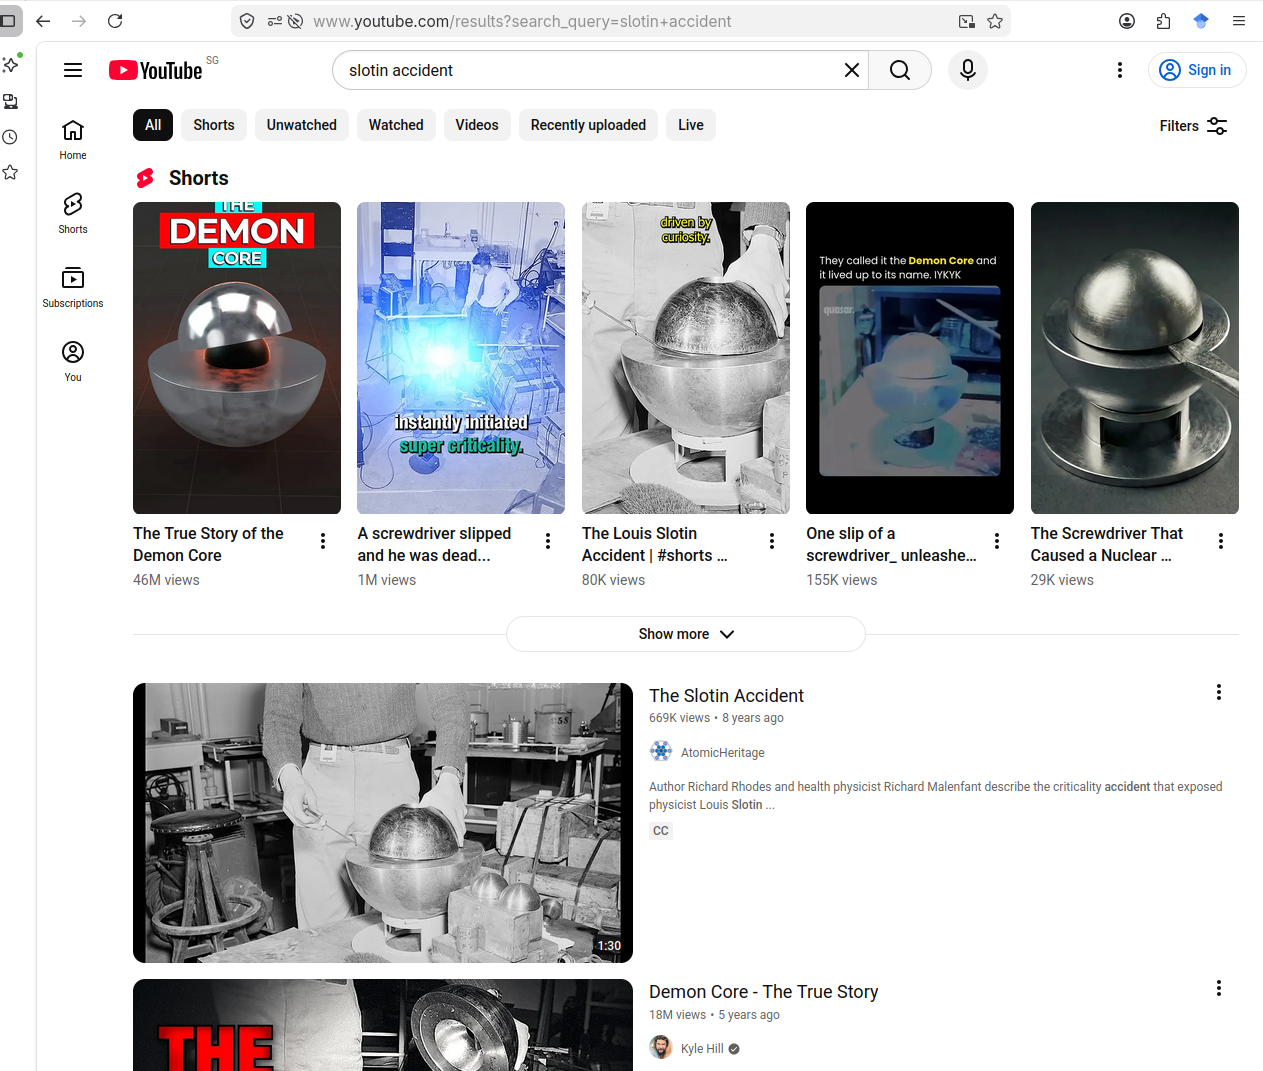
\includegraphics[width=\textwidth, height=0.6\textheight, keepaspectratio]{./slotin_accident.png}
            \tiny{\textit{YouTube Videos of the "Demon Core" experiment setup.}}
        \end{column}
    \end{columns}
\end{frame}

% --- Slide 25: The Slotin Incident (Part 2) ---
\begin{frame}{The Slotin Incident: The Accident}
    At 3:20 PM, Slotin's screwdriver slipped \cite{stratton1989review,oettingen2018criticality}.

    \vspace{1em}
    The hemispheres came together. The core went \textbf{super-prompt critical} instantly—estimated at roughly \textbf{\textdollar 1.10} \cite{oettingen2018criticality}.

    \vspace{1em}
    \textbf{What happened in that instant:}
    \begin{itemize}
        \item Bright flash of blue light (Cherenkov radiation)
        \item Wave of heat across Slotin's hand
        \item Sour taste in his mouth (ionization of air)
        \item Duration: less than one second
    \end{itemize}

    \vspace{1em}
    Slotin immediately knocked the top hemisphere away with his bare hand, stopping the reaction. His quick action likely saved the lives of the seven other people in the room.

    \vspace{1em}
    But the damage was done.
\end{frame}

% --- Slide 26: The Slotin Incident (Part 3) ---
\begin{frame}{The Slotin Incident: The Aftermath}
    \textbf{Radiation dose received:} Estimated 2,100 rad (21 Gy) in less than one second \cite{stratton1989review}.

    \vspace{1em}
    \textbf{Timeline of Louis Slotin's condition:}
    \begin{itemize}
        \item \textbf{Day 1:} Nausea and vomiting began within hours
        \item \textbf{Day 2-3:} Severe radiation burns appeared on his hands
        \item \textbf{Day 4-6:} Mental confusion, loss of coordination
        \item \textbf{Day 7-8:} Internal organs failing, extreme pain
        \item \textbf{Day 9:} Louis Slotin died on May 30, 1946
    \end{itemize}

    \vspace{1em}
    \begin{alertblock}{The Critical Lesson}
        Human reaction time ($\sim$0.25 s) is meaningless when prompt criticality unfolds in microseconds. Even Slotin's heroic reflexes couldn't save him—he had already received a lethal dose before his brain could process what happened.
    \end{alertblock}
\end{frame}

% --- Slide 27: The BORAX Experiments (Part 1) ---
\begin{frame}{The BORAX Experiments: Proving the Danger (1950s)}
    After incidents like Slotin's, the nuclear community needed to understand prompt criticality in \textit{reactor} systems, not just bare cores.

    \vspace{1em}
    \textbf{The Question:} What happens if a water-cooled reactor goes prompt critical?

    \vspace{1em}
    The Boiling Water Reactor Experiments (BORAX) at Idaho National Laboratory were designed to answer this—by deliberately destroying reactors.

    \vspace{1em}
    \begin{block}{The BORAX-I Final Test (July 22, 1954)}
        BORAX-I was built partially underground and operated remotely from a considerable distance. Scientists programmed the reactor to rapidly eject a high-worth control rod, inserting reactivity well above \textdollar 1.00 \cite{putman2012criticality}.
        
        They evacuated everyone to a safe distance and filmed what happened.
    \end{block}
\end{frame}

% --- Slide 28: BORAX-I: The Destruction ---
\begin{frame}{BORAX-I: The Destruction}
    \begin{columns}
        \begin{column}{0.5\textwidth}
            \textbf{Expected outcome} \cite{putman2012criticality}:
            \begin{itemize}
                \item Severe core damage
                \item Fuel melting
                \item Release of $\sim$80 megajoules
                \item Relatively large steam explosion
            \end{itemize}

            \vspace{1em}
            \textbf{Actual outcome:}
            \begin{itemize}
                \item Released $\sim$\textbf{135 megajoules} (69\% more!)
                \item Much more destructive than predicted
                \item Classified as an \textit{accident} due to unexpected severity
            \end{itemize}
        \end{column}
        \begin{column}{0.5\textwidth}
            \centering
			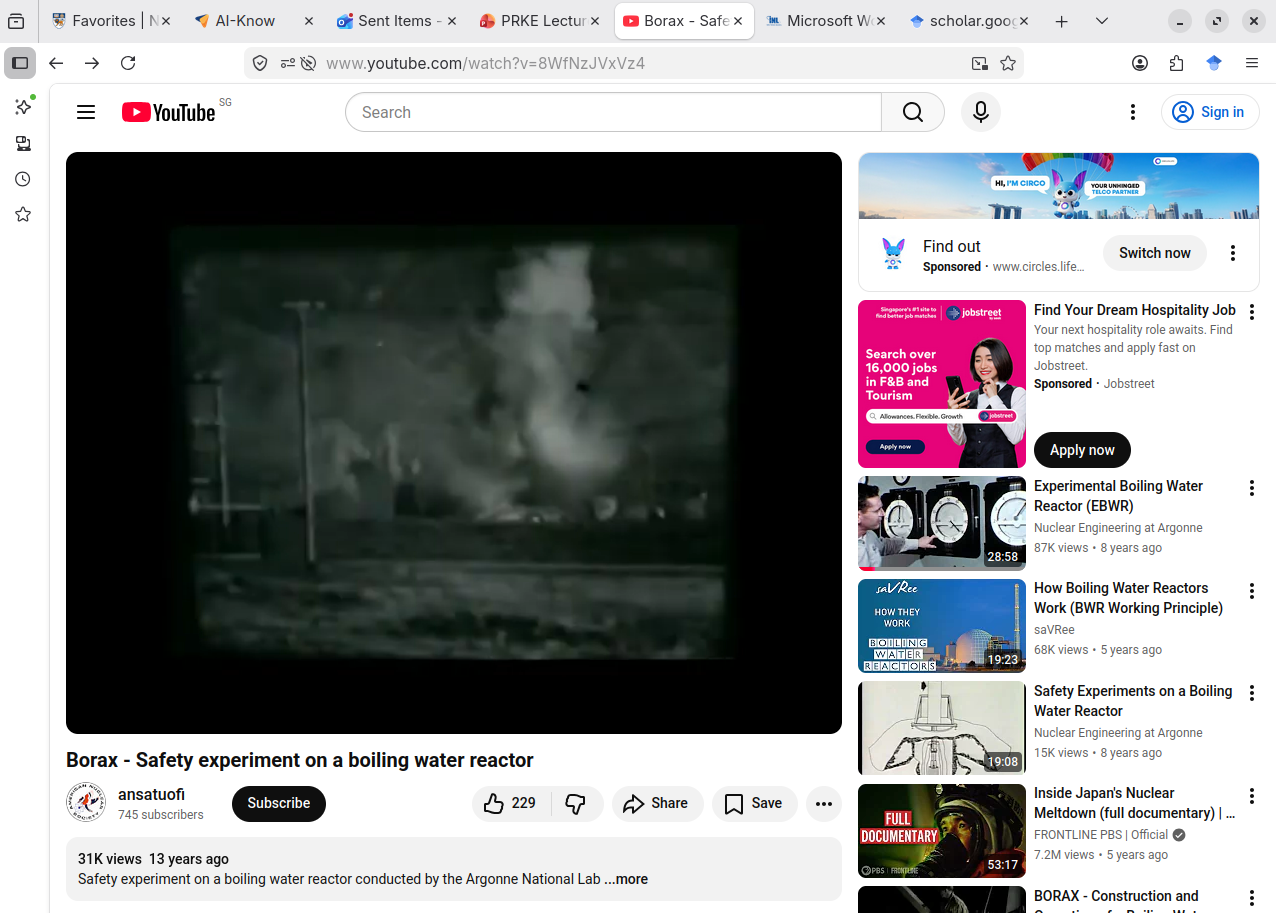
\includegraphics[width=0.9\textwidth, keepaspectratio]{./borax_youtube.png}
            \tiny{\textit{BORAX-I final destructive test - YouTube Video }}
        \end{column}
    \end{columns}
\end{frame}

% --- Slide 29: BORAX-I: Sequence of Destruction ---
\begin{frame}{BORAX-I: Sequence of Destruction}
    \textbf{What happened} \cite{putman2012criticality}:

    \vspace{1em}
    \begin{enumerate}
        \item \textbf{Control rod ejected} – Rapid reactivity insertion (>\textdollar 1.00)
        \item \textbf{Nuclear excursion} – Power rose exponentially in milliseconds
        \item \textbf{Extensive fuel melting} – Direct result of prompt criticality
        \item \textbf{Steam explosion} – Initiated by damage from the criticality
        \item \textbf{Massive destruction:}
        \begin{itemize}
            \item 2,200 lb control rod mechanism thrown 30 feet into the air
            \item Fuel pieces ejected up to 200 feet away
            \item Fortunately, damage was limited to the reactor itself
        \end{itemize}
    \end{enumerate}

    \vspace{1em}
    \href{https://youtu.be/8WfNzJVxVz4?si=vcfWk0Pa0f214-q2&t=790}{\textcolor{blue}{\underline{Watch the BORAX destruction test (YouTube)}}}
    
    \href{https://inldigitallibrary.inl.gov/content/uploads/50/2026/04/5427214.pdf}{\textcolor{blue}{\underline{Read the full INL report (p. 117)}}}
\end{frame}

% --- Slide 30: BORAX: Why Didn't Safety Features Work? ---
\begin{frame}{BORAX: Why Didn't Safety Features Work?}
    Boiling Water Reactors (BWRs) have multiple passive safety features:
    \begin{itemize}
        \item Natural circulation cooling
        \item Negative void coefficient (steam bubbles reduce reactivity)
        \item Negative fuel temperature coefficient
    \end{itemize}

    \vspace{1em}
    \textbf{So why did the reactor explode?}

    \vspace{1em}
    \begin{alertblock}{The Speed Problem}
        Prompt criticality happens in \textbf{milliseconds}. The fuel temperature feedback \textit{did} activate and stop the nuclear reaction—but not before the fuel temperature rose so high that it \textbf{melted the fuel}.
        
        The molten fuel then violently interacted with water, causing a steam explosion that was \textbf{69\% more energetic than predicted}.
        
        Physics worked—but too slowly to prevent catastrophic damage.
    \end{alertblock}
\end{frame}

% --- Slide 31: Can Modern Reactors Survive Prompt Criticality? ---
\begin{frame}{Can Modern Reactors Survive Prompt Criticality?}
    \textbf{It depends on the reactor design and fuel type.}

    \vspace{1em}
    \begin{block}{Light Water Reactors (LWRs) / BWRs}
        \textbf{Negative fuel temperature coefficient stops the reaction quickly.}
        
        However, the fuel temperature can rise so high (\textgreater 2800°C) that the fuel \textbf{melts} before the feedback stops the excursion.
        
        Result: Fuel damage, potential steam explosion (as in BORAX-I \cite{putman2012criticality}).
    \end{block}

    \vspace{1em}
    \textbf{Key issue:} Low thermal margin in UO₂ fuel—melting point is relatively close to operating temperature.
\end{frame}

% --- Slide 32: High-Temperature Reactors: Better Margins ---
\begin{frame}{High-Temperature Reactors: Better Margins}
    \begin{block}{HTGRs (High-Temperature Gas Reactors) and FHRs}
        These reactors use \textbf{TRISO fuel particles}—ceramic-coated fuel designed to withstand extreme temperatures (\textgreater 1600°C).
        
        \textbf{Key advantages:}
        \begin{itemize}
            \item \textbf{Higher thermal margins:} TRISO fuel can tolerate much higher temperatures before failure
            \item \textbf{Strong negative temperature coefficient:} Fuel temperature rise quickly reduces reactivity
            \item \textbf{Lower excess reactivity:} Less potential for large reactivity insertions
        \end{itemize}

        \textbf{Result:} Fuel temperature feedback \textit{may} stop a prompt criticality event without damaging the fuel—\textbf{provided the excess reactivity insertion isn't too large.}
    \end{block}

    This is why HTGRs and FHRs are considered to have superior passive safety characteristics.
\end{frame}

% --- Slide 33: The Bottom Line: Never Go Prompt Critical ---
\begin{frame}{The Bottom Line: Never Go Prompt Critical}
    \textbf{Regardless of reactor type, prompt criticality is unacceptable.}

    \vspace{1em}
    \begin{itemize}
        \item \textbf{LWRs/BWRs:} Prompt criticality leads to fuel melting and potential steam explosions—BORAX-I proved this catastrophically \cite{putman2012criticality}
        \item \textbf{HTGRs/FHRs:} May survive small prompt criticality events, but only if excess reactivity is limited
        \item \textbf{Fast reactors:} Even more sensitive due to shorter neutron lifetimes
    \end{itemize}

    \vspace{1em}
    \begin{alertblock}{The Engineering Rule}
        All reactors are designed with \textbf{reactivity limits} to ensure they can \textit{never} reach \textdollar 1.00 under any credible scenario.
        
        Multiple independent systems (control rods, shutdown systems, reactivity coefficients) provide defense-in-depth.
    \end{alertblock}

    \textbf{This is why you must understand and respect the dollar boundary.}
\end{frame}

% --- Slide 34: Case Study 3: Chernobyl (1986) ---
\begin{frame}{Case Study 3: The Chernobyl Disaster (1986)}
    We've seen two examples of prompt criticality:
    \begin{itemize}
        \item \textbf{Slotin:} Bare critical assembly - instant death
        \item \textbf{BORAX:} BWR with negative feedback - still destroyed
    \end{itemize}

    \vspace{1em}
    \textbf{What about a reactor with positive feedback?}

    \vspace{1em}
    On April 26, 1986, Reactor 4 at the Chernobyl Nuclear Power Plant in Ukraine experienced a catastrophic accident during a turbogenerator safety test \cite{malko2002chernobyl}.

    \vspace{1em}
    \begin{alertblock}{The Result}
        The reactor went prompt critical with \textbf{positive feedback} amplifying the excursion. The explosion completely destroyed the reactor and released massive amounts of radioactive material across Europe, contaminating vast areas for decades.
    \end{alertblock}
\end{frame}

% --- Slide 35: The RBMK Reactor Design ---
\begin{frame}{The RBMK Reactor: A Flawed Design}
    The Chernobyl reactor was an RBMK-1000 (Reaktor Bolshoy Moshchnosti Kanalnyy) - a graphite-moderated, water-cooled channel reactor \cite{malko2002chernobyl}.

    \vspace{1em}
    \textbf{Design characteristics:}
    \begin{itemize}
        \item Graphite moderator (slows neutrons)
        \item Water coolant (removes heat)
        \item Large physical size (11.8 m diameter, 7 m high core)
        \item Nominal thermal power: 3,200 MWth
        \item Positive steam-void coefficient at low power
    \end{itemize}

    \vspace{1em}
    \begin{alertblock}{The Fatal Flaw: Positive Steam-Void Coefficient}
        In most reactors (LWRs, BWRs), water acts as both coolant \textit{and} moderator. Steam bubbles (voids) reduce moderation $\rightarrow$ reactivity decreases (negative feedback).
        
        In RBMK, graphite is the moderator. Steam voids remove neutron-absorbing water $\rightarrow$ reactivity \textbf{increases} (positive feedback)! The coefficient could reach up to 5$\beta$ at certain conditions.
    \end{alertblock}
\end{frame}

% --- Slide 36: Positive Void Coefficient Explained ---
\begin{frame}{Understanding Positive Steam-Void Coefficient}
    \textbf{Normal reactor (negative void coefficient):}
    \begin{enumerate}
        \item Power increases $\rightarrow$ water heats up $\rightarrow$ steam forms
        \item Steam has lower density $\rightarrow$ less moderation
        \item Less moderation $\rightarrow$ fewer thermal neutrons $\rightarrow$ power decreases (stabilizing)
    \end{enumerate}

    \vspace{1em}
    \textbf{RBMK reactor (positive steam-void coefficient):}
    \begin{enumerate}
        \item Power increases $\rightarrow$ water heats up $\rightarrow$ steam forms
        \item Steam has lower density $\rightarrow$ less neutron absorption in water
        \item Less absorption $\rightarrow$ more neutrons available $\rightarrow$ power \textbf{increases further} (destabilizing)
    \end{enumerate}

    \vspace{1em}
    This creates a \textbf{positive feedback loop}: more power $\rightarrow$ more steam $\rightarrow$ more power $\rightarrow$ more steam...

    \vspace{1em}
    The RBMK's positive steam-void coefficient was particularly dangerous at low power operation \cite{malko2002chernobyl}.
\end{frame}

% --- Slide 37: The Chernobyl Accident Sequence ---
\begin{frame}{What Happened at Chernobyl}
    \begin{columns}
        \begin{column}{0.55\textwidth}
            \textbf{The Setup} \cite{malko2002chernobyl}:
            \begin{itemize}
                \item Turbogenerator test during planned shutdown
                \item Power reduced: 3,200 MW $\rightarrow$ 1,500 MW $\rightarrow$ target 720 MWth
                \item ECCS switched off at 14:00 on April 25
            \end{itemize}

            \vspace{0.5em}
            \textbf{Critical Mistake (00:28, April 26):}
            \begin{itemize}
                \item Power dropped uncontrollably to 30 MWth
                \item Strong xenon poisoning occurred
                \item Deputy chief engineer Dyatlov \textbf{ordered} operators to withdraw nearly all control rods to raise power
                \item Operative reactivity surplus: only 6-8 rods (far below safety limit)
            \end{itemize}
        \end{column}
        \begin{column}{0.45\textwidth}
            \centering
            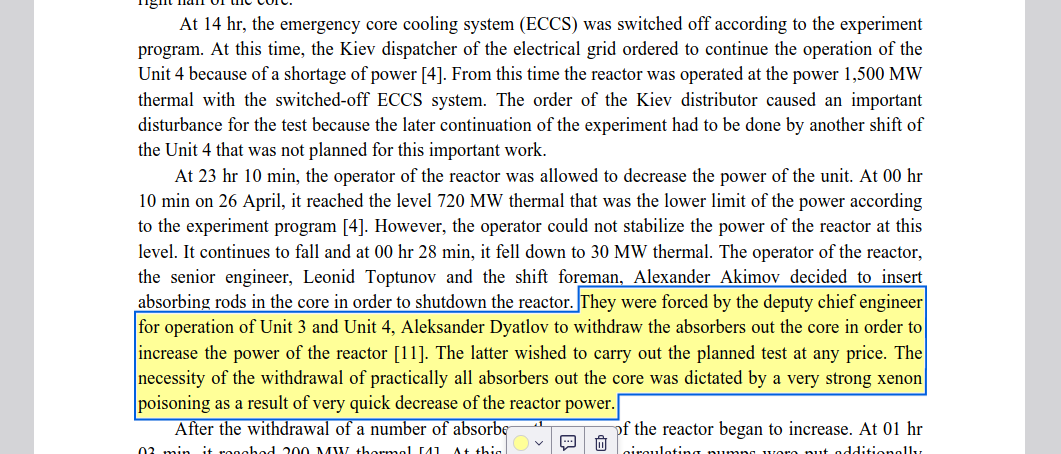
\includegraphics[width=\textwidth, keepaspectratio]{./chernobyl_dyatlov_control_rod_from_core.png}
            \tiny{\textit{Control rod withdrawal beyond safety limits \cite{malko2002chernobyl}}}
        \end{column}
    \end{columns}
\end{frame}

% --- Slide 38: The Fatal Sequence ---
\begin{frame}{The Fatal Sequence (01:23, April 26, 1986)}
    With nearly all control rods withdrawn, the reactor was in an extremely dangerous state \cite{malko2002chernobyl}:
    
    \vspace{0.5em}
    \textbf{01:23:04 - Test initiated:}
    \begin{enumerate}
        \item Turbine valves closed $\rightarrow$ coolant flow decreased slightly
        \item Small power increase began
        \item Power increase $\rightarrow$ steam formation $\rightarrow$ \textbf{positive void feedback activated}
        \item Reactivity increased rapidly $\rightarrow$ power surged uncontrollably
    \end{enumerate}
    
    \vspace{0.5em}
    \textbf{01:23:40 - SCRAM attempted (36 seconds later):}
    \begin{itemize}
        \item Operators pressed AZ-5 (emergency shutdown) button
        \item All control rods began inserting into core
        \item \textbf{Design flaw:} Graphite displacers at rod tips initially \textit{added positive reactivity} ("positive reactivity surge")
        \item Combined with positive void coefficient $\rightarrow$ catastrophic power excursion
    \end{itemize}
    
    \vspace{0.5em}
    \textbf{01:23:47 - Destruction (6-7 seconds after SCRAM):}
    Reactor destroyed by explosions before rods could fully insert.
\end{frame}

% --- Slide 39: The Explosion and Aftermath ---
\begin{frame}{The Chernobyl Explosion}
    \begin{columns}
        \begin{column}{0.5\textwidth}
            \textbf{The Explosions} \cite{malko2002chernobyl}:
            \begin{itemize}
                \item At least two explosions occurred
                \item First: likely steam explosion
                \item Second: possibly nuclear explosion (estimated 200 tons TNT equivalent)
                \item Core completely destroyed
                \item 2,000 ton upper structure thrown upward
                \item Graphite fire released radioactive material for 10 days
            \end{itemize}

            \vspace{1em}
            \textbf{Why feedback didn't save it:}
            Positive void coefficient \textit{amplified} the excursion. By the time negative fuel temperature feedback could activate, the reactor was already destroyed.
        \end{column}
        \begin{column}{0.5\textwidth}
            \centering
			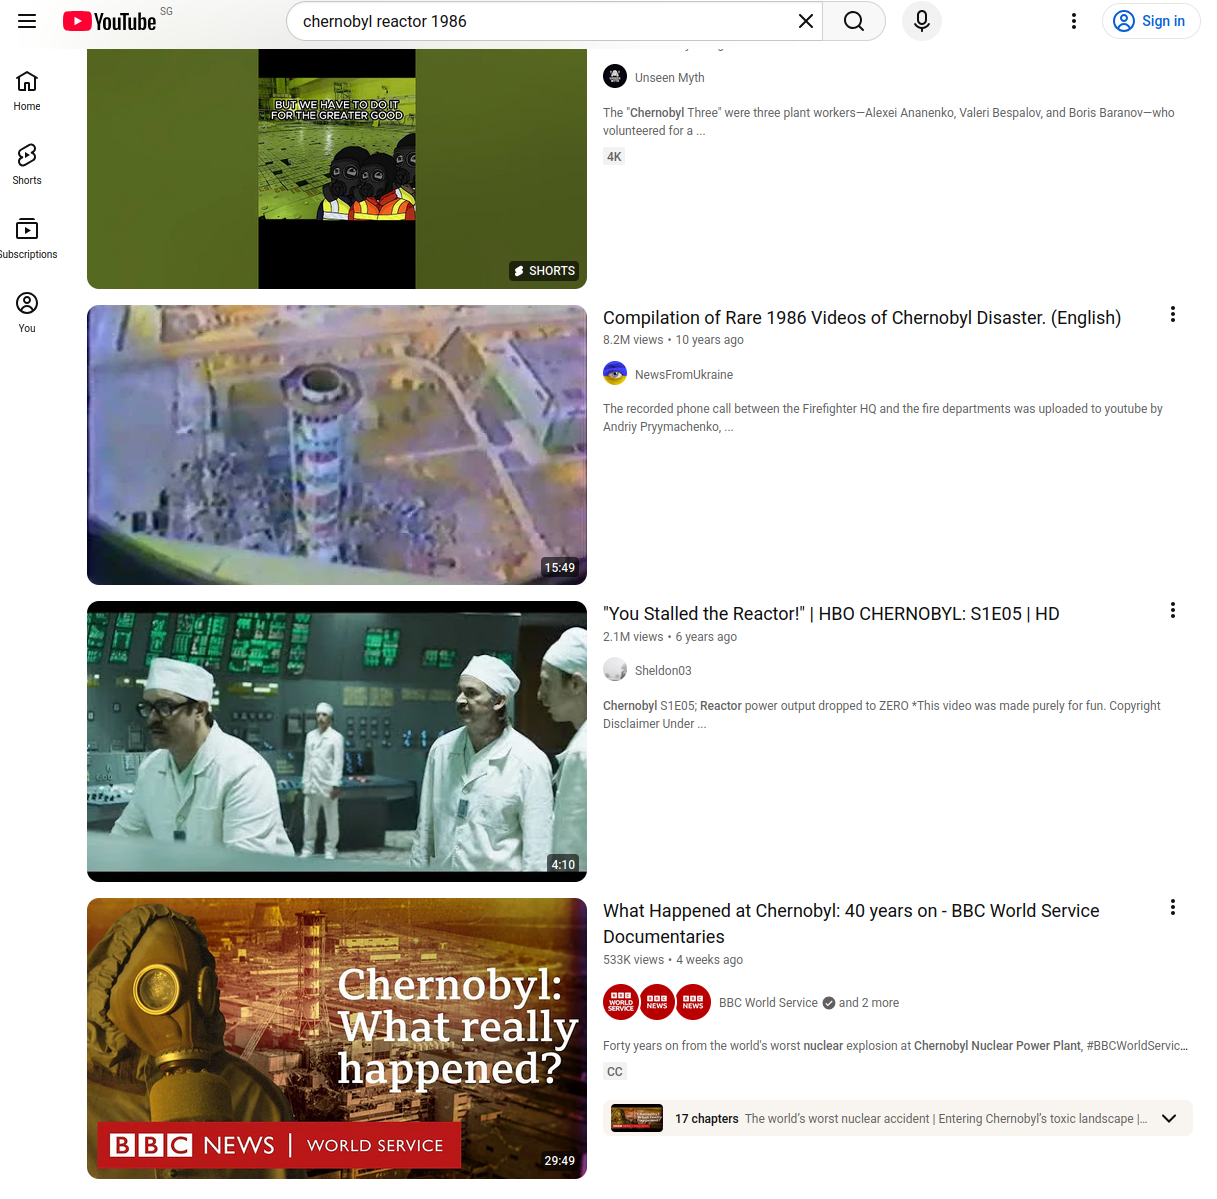
\includegraphics[width=0.9\textwidth, keepaspectratio]{./chernobyl_youtube.png}
            \tiny{\textit{Chernobyl Reactor 4 after the explosion.}}
            
            \vspace{1em}
            \href{https://www.rri.kyoto-u.ac.jp/NSRG/reports/kr79/kr79pdf/Malko1.pdf}{\textcolor{blue}{\underline{Read detailed analysis (Malko, 2002)}}}
        \end{column}
    \end{columns}
\end{frame}

% --- Slide 40: Lessons from Chernobyl ---
\begin{frame}{Lessons from Chernobyl}
    \textbf{Design Lessons} \cite{malko2002chernobyl}:
    \begin{itemize}
        \item \textbf{Never design reactors with positive void/steam coefficients}
        \item All modern reactors require negative reactivity coefficients
        \item Control rods must always add negative reactivity when inserted (no "positive reactivity surge")
        \item Adequate shutdown margin must be maintained at all times
        \item Proper documentation and understanding of reactor limitations essential
    \end{itemize}
    
    \vspace{0.5em}
    \textbf{Operational Lessons:}
    \begin{itemize}
        \item Safety systems must not be disabled during tests
        \item Operators must understand reactor physics (especially feedback mechanisms)
        \item Low-power operation in unstable configurations is extremely dangerous
        \item Nuclear safety culture must prioritize safety over completing tests
    \end{itemize}

    \vspace{0.5em}
    \begin{block}{The Common Thread}
        Slotin, BORAX, and Chernobyl all demonstrate: \textbf{prompt criticality is catastrophic}. Even "safety features" like feedback can make things worse if they're positive instead of negative.
    \end{block}
\end{frame}

% --- Slide 41: Comparing the Three Cases ---
\begin{frame}{Three Accidents: Three Lessons}
    \small
    \begin{tabular}{p{2.5cm}p{3.2cm}p{3.2cm}p{3.8cm}}
        \toprule
        \textbf{Accident} & \textbf{System} & \textbf{Feedback} & \textbf{Outcome} \\
        \midrule
        \textbf{Slotin (1946)} & Bare Pu core & None & Prompt critical $\rightarrow$ instant lethal dose. Human reaction time irrelevant. \\
        \addlinespace
        \textbf{BORAX (1954)} & BWR with UO$_2$ fuel & Negative (fuel temp.) & Feedback stopped reaction, but fuel melted first $\rightarrow$ steam explosion. \\
        \addlinespace
        \textbf{Chernobyl (1986)} & RBMK reactor & \textbf{Positive} (steam-void) & Feedback \textit{amplified} excursion $\rightarrow$ catastrophic destruction. \\
        \bottomrule
    \end{tabular}

    \vspace{1em}
\end{frame}

% --- Slide 42: The Universal Rule ---
\begin{frame}{The Universal Rule}
    \textbf{The Universal Rule:}
    \begin{itemize}
        \item Prompt criticality must be prevented by design
        \item Negative feedback helps, but isn't fast enough to prevent damage
        \item Positive feedback is absolutely unacceptable
        \item Multiple independent safety systems are essential
    \end{itemize}
\end{frame}

% --- Slide 43: Acknowledgments ---
\begin{frame}{Acknowledgments}
    \begin{block}{Development of These Materials}
        This presentation was developed with assistance from \textbf{NUS AI-Know}, 
        the National University of Singapore's trusted generative AI platform 
        \cite{aiknow2025prke}
    \end{block}

    \vspace{1em}
    \textbf{AI-Know Platform:}
    \begin{itemize}
        \item Secure, compliant AI environment aligned with NUS policies
        \item Conversational AI for educational content development
        \item Private interactions that are never used to train models
    \end{itemize}

    \vspace{1em}
    \textbf{Special Thanks:}
    \begin{itemize}
        \item NUS SNRSI, for their support in enabling me to develop 
            Outram Park (Open source Unified TRAnsient Multi Phase 
            Advanced Reactor simulation Kit)
        \item Historical documentation sources (Los Alamos, INL, Kyoto University)
    \end{itemize}

    \vspace{1em}
    \centering
    \small
    \textit{For more information about AI-Know: \href{https://ai-know.nus.edu.sg}{https://ai-know.nus.edu.sg}}
\end{frame}

\begin{frame}[allowframebreaks]{References}
    \printbibliography[heading=none]
\end{frame}

\end{document}
